\documentclass[11pt,a4paper]{article}

\usepackage[margin=20mm,headheight=15pt]{geometry}

\usepackage{longtable,booktabs,array,hyperref,xcolor,tikz,fancyhdr}

\usepackage{fontspec,xeCJK}

\setmainfont[Ligatures=TeXOff]{Times New Roman}

\setsansfont[Ligatures=TeXOff]{Times New Roman}

\setmonofont[Ligatures=TeXOff,WordSpace={1,1,1}]{Times New Roman}

\setCJKmainfont{Noto Serif CJK SC}

\setCJKsansfont{Noto Serif CJK SC}

\setCJKmonofont{Noto Serif CJK SC}

\newfontfamily\vulcanmathsymbols{Noto Serif CJK SC}

\XeTeXgenerateactualtext=1

\definecolor{vulcan}{HTML}{BB3E23}

\pgfdeclarelayer{connections}\pgfdeclarelayer{edge labels}\pgfsetlayers{connections,main,edge labels}

\hypersetup{hidelinks}

\newcolumntype{L}[1]{>{\raggedright\arraybackslash}p{#1}}

\setlength{\emergencystretch}{5em}\tolerance=2000\hbadness=10000

\setlength{\parindent}{0pt}\setlength{\parskip}{5pt}

\pagestyle{fancy}\fancyhf{}\fancyhead[L]{\small\sffamily\textbf{VULCAN SILICON ENGINEERING}}

\fancyhead[R]{\small\sffamily Technical Design, Quartus STA \& FPGA Verification Report}\fancyfoot[C]{\small\sffamily Page \thepage}

\begin{document}

{\footnotesize\sffamily\textcolor{vulcan}{\textbf{VULCAN AUTONOMOUS CHIP DESIGN \& HARDWARE SIGNOFF SERIES \hfill DOCUMENT CLASS: ENGINEERING VERIFICATION REPORT}}\par}

\vspace{2pt}\textcolor{vulcan}{\rule{\textwidth}{1.2pt}}\vspace{4pt}

{\sffamily\LARGE\raggedright\textbf{BILLET-F3: Programmable Four-Channel FIR/\allowbreak{}SOS Filter Chain}\par}

\vspace{4pt}

{\footnotesize\sffamily\renewcommand{\arraystretch}{1.22}\begin{tabular}{@{}L{0.22\textwidth}L{0.74\textwidth}@{}}\toprule\textbf{Author \& Contact} & Sufeng Guo (\allowbreak{}sufeng\_\allowbreak{}guo@smail.nju.edu.cn,\allowbreak{} v-sufengguo@microsoft.com)\allowbreak{}\\\textbf{Target Platform} & Intel Arria 10 GX (\texttt{10AX115N3F40E2SG}) \textemdash{} Microsoft Catapult Longs Peak (Bedrock 2.1)\\\textbf{Verification Stack} & Icarus Verilog 12.0 $\cdot$ Yosys 0.33 $\cdot$ Intel Quartus Prime 17.1 TimeQuest STA $\cdot$ PCIe Gen3x8 HIL\\\textbf{Release Timestamp} & 2026-10-19 23:40 UTC+\allowbreak{}8 (\allowbreak{}Beijing Time)\allowbreak{}\\\bottomrule\end{tabular}\par}

\vspace{4pt}

\begin{abstract}\noindent 

BILLET-F3 is synthesizable SystemVerilog filter IP with top module \texttt{billet\_\allowbreak{}f3\_\allowbreak{}top}. It preserves the supplied programmable four-channel FIR and adds a shared recursive second-order-section engine supporting one to four sections. A global descriptor selects registered bypass,\allowbreak{} FIR,\allowbreak{} SOS,\allowbreak{} FIR followed by SOS,\allowbreak{} or SOS followed by FIR; coefficients and histories remain channel-specific.


Independent Icarus execution compared 550,\allowbreak{}300 retired behavioral samples and 4,\allowbreak{}533,\allowbreak{}760 numerical samples without mismatches. Across 42 fixture/\allowbreak{}order response cases,\allowbreak{} the worst normalized time-domain error was 3.112162e-5 and the worst complex frequency-response error was 5.493164e-4. Four injected RTL defects were detected,\allowbreak{} five configurations passed Yosys synthesis and structural assertions,\allowbreak{} and bounded clean-directory reproduction executed successfully. These results establish finite-precision RTL behavior and generic synthesizability,\allowbreak{} not physical implementation performance.


\end{abstract}

\section{Architecture and design rationale}

The wrapper routes one outstanding transaction through an unchanged FIR instance and a sequential SOS engine. Retaining the five parent modules byte-for-byte preserves arithmetic,\allowbreak{} coefficient banking,\allowbreak{} history and default cycle behavior. The SOS engine executes one section per cycle with five parallel signed multipliers; it shares arithmetic across sections and channels rather than replicating section pipelines. Mixed modes transfer the first block's registered result to the second on the following edge. Final outputs expose existing child registers,\allowbreak{} avoiding an extra wrapper latency stage. The delivered RTL comprises nine modules,\allowbreak{} 936 lines and 38,\allowbreak{}003 bytes [\allowbreak{}E001,\allowbreak{} E003–E011,\allowbreak{} E034]\allowbreak{}.

\begin{center}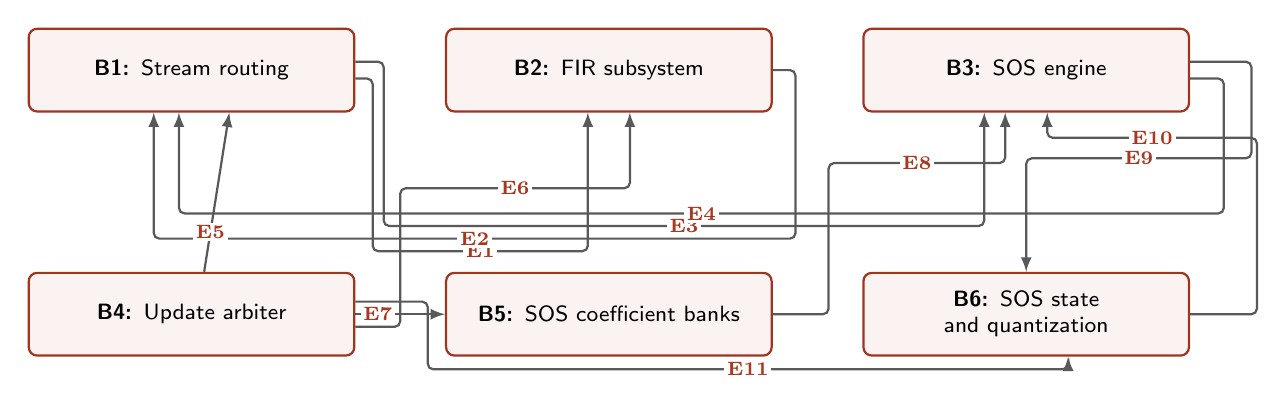
\begin{tikzpicture}[every node/.style={font=\footnotesize\sffamily},>=latex]

\node[draw=vulcan!85!black,thick,rounded corners=3pt,fill=vulcan!6,text width=3.9cm,minimum height=1.05cm,align=center] (b0) at (0.0,0.0) {\textbf{B1:} Stream routing};

\node[draw=vulcan!85!black,thick,rounded corners=3pt,fill=vulcan!6,text width=3.9cm,minimum height=1.05cm,align=center] (b1) at (5.3,0.0) {\textbf{B2:} FIR subsystem};

\node[draw=vulcan!85!black,thick,rounded corners=3pt,fill=vulcan!6,text width=3.9cm,minimum height=1.05cm,align=center] (b2) at (10.6,0.0) {\textbf{B3:} SOS engine};

\node[draw=vulcan!85!black,thick,rounded corners=3pt,fill=vulcan!6,text width=3.9cm,minimum height=1.05cm,align=center] (b3) at (0.0,-3.1) {\textbf{B4:} Update arbiter};

\node[draw=vulcan!85!black,thick,rounded corners=3pt,fill=vulcan!6,text width=3.9cm,minimum height=1.05cm,align=center] (b4) at (5.3,-3.1) {\textbf{B5:} SOS coefficient banks};

\node[draw=vulcan!85!black,thick,rounded corners=3pt,fill=vulcan!6,text width=3.9cm,minimum height=1.05cm,align=center] (b5) at (10.6,-3.1) {\textbf{B6:} SOS state and quantization};

\begin{pgfonlayer}{connections}

\draw[->,thick,black!65,rounded corners=2pt] ([yshift=-0.107cm]b0.east) -- (2.300,-0.107) -- (2.300,-2.300) -- coordinate[midway] (e0) (5.033,-2.300) -- ([xshift=-0.267cm]b1.south);

\draw[->,thick,black!65,rounded corners=2pt] ([yshift=0.000cm]b1.east) -- (7.670,0.000) -- (7.670,-2.140) -- coordinate[midway] (e1) (-0.480,-2.140) -- ([xshift=-0.480cm]b0.south);

\draw[->,thick,black!65,rounded corners=2pt] ([yshift=0.107cm]b0.east) -- (2.440,0.107) -- (2.440,-1.980) -- coordinate[midway] (e2) (10.067,-1.980) -- ([xshift=-0.533cm]b2.south);

\draw[->,thick,black!65,rounded corners=2pt] ([yshift=-0.107cm]b2.east) -- (13.110,-0.107) -- (13.110,-1.820) -- coordinate[midway] (e3) (-0.160,-1.820) -- ([xshift=-0.160cm]b0.south);

\draw[->,thick,black!65] ([xshift=0.160cm]b3.north) -- coordinate[pos=0.25] (e4) ([xshift=0.480cm]b0.south);

\draw[->,thick,black!65,rounded corners=2pt] ([yshift=-0.160cm]b3.east) -- (2.650,-3.260) -- (2.650,-1.500) -- coordinate[midway] (e5) (5.567,-1.500) -- ([xshift=0.267cm]b1.south);

\draw[->,thick,black!65] ([yshift=0.000cm]b3.east) -- coordinate[pos=0.25] (e6) ([yshift=0.000cm]b4.west);

\draw[->,thick,black!65,rounded corners=2pt] ([yshift=0.000cm]b4.east) -- (8.090,-3.100) -- (8.090,-1.180) -- coordinate[midway] (e7) (10.333,-1.180) -- ([xshift=-0.267cm]b2.south);

\draw[->,thick,black!65,rounded corners=2pt] ([yshift=0.107cm]b2.east) -- (13.460,0.107) -- (13.460,-1.120) -- coordinate[midway] (e8) (10.600,-1.120) -- ([xshift=0.000cm]b5.north);

\draw[->,thick,black!65,rounded corners=2pt] ([yshift=0.000cm]b5.east) -- (13.530,-3.100) -- (13.530,-0.860) -- coordinate[midway] (e9) (10.867,-0.860) -- ([xshift=0.267cm]b2.south);

\draw[->,thick,black!65,rounded corners=2pt] ([yshift=0.160cm]b3.east) -- (3.000,-2.940) -- (3.000,-3.800) -- coordinate[midway] (e10) (11.133,-3.800) -- ([xshift=0.533cm]b5.south);

\end{pgfonlayer}

\begin{pgfonlayer}{edge labels}

\node[fill=white,inner sep=1pt,font=\scriptsize\bfseries,text=vulcan!90!black] at (e0) {E1};

\node[fill=white,inner sep=1pt,font=\scriptsize\bfseries,text=vulcan!90!black] at (e1) {E2};

\node[fill=white,inner sep=1pt,font=\scriptsize\bfseries,text=vulcan!90!black] at (e2) {E3};

\node[fill=white,inner sep=1pt,font=\scriptsize\bfseries,text=vulcan!90!black] at (e3) {E4};

\node[fill=white,inner sep=1pt,font=\scriptsize\bfseries,text=vulcan!90!black] at (e4) {E5};

\node[fill=white,inner sep=1pt,font=\scriptsize\bfseries,text=vulcan!90!black] at (e5) {E6};

\node[fill=white,inner sep=1pt,font=\scriptsize\bfseries,text=vulcan!90!black] at (e6) {E7};

\node[fill=white,inner sep=1pt,font=\scriptsize\bfseries,text=vulcan!90!black] at (e7) {E8};

\node[fill=white,inner sep=1pt,font=\scriptsize\bfseries,text=vulcan!90!black] at (e8) {E9};

\node[fill=white,inner sep=1pt,font=\scriptsize\bfseries,text=vulcan!90!black] at (e9) {E10};

\node[fill=white,inner sep=1pt,font=\scriptsize\bfseries,text=vulcan!90!black] at (e10) {E11};

\end{pgfonlayer}

\end{tikzpicture}\par

{\small\textbf{Figure 1:} Top-level microarchitectural functional block map and directed inter-module bus topology.}\end{center}

{\small\renewcommand{\arraystretch}{1.18}\begin{longtable}{@{}L{0.24\textwidth}L{0.7\textwidth}@{}}\toprule

\textbf{Block} & \textbf{Responsibility}\\\midrule\endhead

B1: Stream routing & Input/\allowbreak{}output selection,\allowbreak{} registered bypass and a single transaction reservation; permits simultaneous final retirement and next-sample acceptance.\\[3pt]

B2: FIR subsystem & Literal \texttt{u\_\allowbreak{}fir} instance of \texttt{billet\_\allowbreak{}f2\_\allowbreak{}top},\allowbreak{} retaining coefficient-bank,\allowbreak{} history,\allowbreak{} grouped MAC and rounding submodules.\\[3pt]

B3: SOS engine & Literal \texttt{u\_\allowbreak{}sos} instance; executes the ascending active section prefix using direct form I and channel-isolated recursive state.\\[3pt]

B4: Update arbiter & Installs legal global descriptors and admits quiescent commits with chain,\allowbreak{} SOS-commit,\allowbreak{} FIR-commit priority.\\[3pt]

B5: SOS coefficient banks & Two banks per channel,\allowbreak{} five signed coefficients per physical section,\allowbreak{} completeness masks and active-bank selectors.\\[3pt]

B6: SOS state and quantization & Per-channel/\allowbreak{}per-section x1,\allowbreak{} x2,\allowbreak{} y1,\allowbreak{} y2 storage; convergent rounding and saturation at recursive and external boundaries.\\[3pt]

\bottomrule\end{longtable}}

{\small\renewcommand{\arraystretch}{1.18}\begin{longtable}{@{}L{0.24\textwidth}L{0.7\textwidth}@{}}\toprule

\textbf{Directed relationship} & \textbf{Meaning}\\\midrule\endhead

E1: B1 to B2 & Accepted sample or routed SOS result\\[3pt]

E2: B2 to B1 & Registered FIR result\\[3pt]

E3: B1 to B3 & Accepted sample or routed FIR result\\[3pt]

E4: B3 to B1 & Registered SOS result\\[3pt]

E5: B4 to B1 & Descriptor and acceptance gating\\[3pt]

E6: B4 to B2 & Quiescent FIR commit\\[3pt]

E7: B4 to B5 & Quiescent SOS bank commit\\[3pt]

E8: B5 to B3 & Selected channel/\allowbreak{}bank/\allowbreak{}section coefficients\\[3pt]

E9: B3 to B6 & Accumulator and simultaneous state update\\[3pt]

E10: B6 to B3 & Old histories and quantized result\\[3pt]

E11: B4 to B6 & Global or channel-specific state clear\\[3pt]

\bottomrule\end{longtable}}

\section{Interfaces and configuration}

{\small\renewcommand{\arraystretch}{1.18}\begin{longtable}{@{}L{0.2\textwidth}L{0.12\textwidth}L{0.1\textwidth}L{0.48\textwidth}@{}}\toprule

\textbf{Signal /\allowbreak{} group} & \textbf{Direction} & \textbf{Width} & \textbf{Contract}\\\midrule\endhead

clk,\allowbreak{} rst\_\allowbreak{}n & Input & 1 bit each & Single clock domain; rising-edge handshakes and asynchronous active-low reset.\\[3pt]

s\_\allowbreak{}data,\allowbreak{} s\_\allowbreak{}channel,\allowbreak{} s\_\allowbreak{}valid; s\_\allowbreak{}ready & Input; output ready & Signed 16-bit data,\allowbreak{} 2-bit channel,\allowbreak{} 1-bit valid/\allowbreak{}ready & Accepts a sample when pre-edge valid and ready are both asserted. Channels are 0 through 3.\\[3pt]

m\_\allowbreak{}data,\allowbreak{} m\_\allowbreak{}channel,\allowbreak{} m\_\allowbreak{}valid; m\_\allowbreak{}ready & Output; input ready & Signed 16-bit data,\allowbreak{} 2-bit channel,\allowbreak{} 1-bit valid/\allowbreak{}ready & Preserves accepted ordering and channel identity. Valid data/\allowbreak{}channel remain stable under backpressure; invalid data/\allowbreak{}channel are zero.\\[3pt]

cfg\_\allowbreak{}valid,\allowbreak{} cfg\_\allowbreak{}channel,\allowbreak{} cfg\_\allowbreak{}addr,\allowbreak{} cfg\_\allowbreak{}data; cfg\_\allowbreak{}ready & Input; output ready & 1,\allowbreak{} 2,\allowbreak{} ADDR\_\allowbreak{}W,\allowbreak{} signed 16; 1 bit & Writes the selected channel's inactive FIR bank. ADDR\_\allowbreak{}W=\allowbreak{}max(\allowbreak{}1,\allowbreak{}ceil(\allowbreak{}log2(\allowbreak{}TAP\_\allowbreak{}COUNT)\allowbreak{})\allowbreak{})\allowbreak{}; only addresses below TAP\_\allowbreak{}COUNT are accepted.\\[3pt]

commit\_\allowbreak{}valid,\allowbreak{} commit\_\allowbreak{}channel; commit\_\allowbreak{}ready & Input; output ready & 1,\allowbreak{} 2; 1 bit & Requests a complete inactive FIR-bank swap at a globally empty boundary.\\[3pt]

sos\_\allowbreak{}cfg\_\allowbreak{}valid,\allowbreak{} sos\_\allowbreak{}cfg\_\allowbreak{}channel,\allowbreak{} sos\_\allowbreak{}cfg\_\allowbreak{}section,\allowbreak{} sos\_\allowbreak{}cfg\_\allowbreak{}addr,\allowbreak{} sos\_\allowbreak{}cfg\_\allowbreak{}data; sos\_\allowbreak{}cfg\_\allowbreak{}ready & Input; output ready & 1,\allowbreak{} 2,\allowbreak{} 2,\allowbreak{} 3,\allowbreak{} signed 18; 1 bit & Writes inactive SOS coefficients. Section must be below SOS\_\allowbreak{}COUNT; addresses 0–4 select b0,\allowbreak{} b1,\allowbreak{} b2,\allowbreak{} a1,\allowbreak{} a2.\\[3pt]

sos\_\allowbreak{}commit\_\allowbreak{}valid,\allowbreak{} sos\_\allowbreak{}commit\_\allowbreak{}channel; sos\_\allowbreak{}commit\_\allowbreak{}ready & Input; output ready & 1,\allowbreak{} 2; 1 bit & Swaps a complete SOS bank for one channel and clears that channel's recursive states.\\[3pt]

chain\_\allowbreak{}valid,\allowbreak{} chain\_\allowbreak{}mode,\allowbreak{} chain\_\allowbreak{}sections; chain\_\allowbreak{}ready & Input; output ready & 1,\allowbreak{} 3,\allowbreak{} 3; 1 bit & Programs the global chain. Modes 0/\allowbreak{}1 are bypass/\allowbreak{}FIR and require zero sections. Modes 2/\allowbreak{}3/\allowbreak{}4 are SOS/\allowbreak{}FIR{\vulcanmathsymbols →}SOS/\allowbreak{}SOS{\vulcanmathsymbols →}FIR and require 1 through SOS\_\allowbreak{}COUNT sections. Other descriptors never handshake.\\[3pt]

\bottomrule\end{longtable}}

{\small\renewcommand{\arraystretch}{1.18}\begin{longtable}{@{}L{0.23\textwidth}L{0.12\textwidth}L{0.57\textwidth}@{}}\toprule

\textbf{Parameter} & \textbf{Default} & \textbf{Meaning /\allowbreak{} supported values}\\\midrule\endhead

TAP\_\allowbreak{}COUNT & 32 & Supported values: 1,\allowbreak{} 8,\allowbreak{} 16,\allowbreak{} 32,\allowbreak{} 64. Defines FIR length independently for each of four channels.\\[3pt]

MAC\_\allowbreak{}LANES & 1 & Supported values: 1,\allowbreak{} 2,\allowbreak{} 4. Excess lanes at TAP\_\allowbreak{}COUNT=\allowbreak{}1 contribute zero.\\[3pt]

SOS\_\allowbreak{}COUNT & 2 & Supported values: 1,\allowbreak{} 2,\allowbreak{} 3,\allowbreak{} 4. Defines physical sections; runtime selection enables an ascending prefix.\\[3pt]

\bottomrule\end{longtable}}

\section{Behavior and corner cases}

\subsection{Exact arithmetic}

External samples and FIR coefficients use signed 16-bit codes scaled by 2\textasciicircum{}-15,\allowbreak{} representing [\allowbreak{}-1,\allowbreak{}1-2\textasciicircum{}-15]\allowbreak{}. FIR retains full products,\allowbreak{} a 32+\allowbreak{}ceil(\allowbreak{}log2(\allowbreak{}TAP\_\allowbreak{}COUNT)\allowbreak{})\allowbreak{}-bit sum,\allowbreak{} rounding right 15 and signed-16 saturation. SOS coefficients are signed 18-bit codes scaled by 2\textasciicircum{}-16,\allowbreak{} representing [\allowbreak{}-2,\allowbreak{}2-2\textasciicircum{}-16]\allowbreak{}. Recursive states are signed 32-bit codes scaled by 2\textasciicircum{}-23,\allowbreak{} representing [\allowbreak{}-256,\allowbreak{}256-2\textasciicircum{}-23]\allowbreak{}. External inputs are promoted by an exact left shift of eight [\allowbreak{}E002,\allowbreak{} E005,\allowbreak{} E006,\allowbreak{} E010]\allowbreak{}.

\subsection{Recursive update and quantization}

Each section computes A=\allowbreak{}b0*\allowbreak{}x+\allowbreak{}b1*\allowbreak{}x1+\allowbreak{}b2*\allowbreak{}x2-a1*\allowbreak{}y1-a2*\allowbreak{}y2 with implicit a0=\allowbreak{}1. Signed 50-bit products are extended before accumulation into 53 bits. The conservative bound 5*\allowbreak{}2\textasciicircum{}48<2\textasciicircum{}51 fits signed 53 bits without intermediate wrap. Round A right 16,\allowbreak{} saturate to signed 32 bits,\allowbreak{} then simultaneously store x2=\allowbreak{}old x1,\allowbreak{} x1=\allowbreak{}x,\allowbreak{} y2=\allowbreak{}old y1,\allowbreak{} y1=\allowbreak{}saturated y. Pass y directly to the next section. Only the cascade boundary rounds right eight and saturates to signed 16 bits. Rounding uses floor quotient/\allowbreak{}remainder with nearest ties-to-even,\allowbreak{} including negative ties; saturation follows rounding [\allowbreak{}E002,\allowbreak{} E008,\allowbreak{} E010]\allowbreak{}.

\subsection{Reset and transaction isolation}

Reset immediately suppresses all public ready/\allowbreak{}valid outputs and zeros output data/\allowbreak{}channel. It aborts traffic and clears both coefficient banks,\allowbreak{} selectors,\allowbreak{} masks,\allowbreak{} histories,\allowbreak{} recursive state and reservations; the descriptor returns to FIR-only. There is exactly one unfinished top-level sample. Computation can finish while downstream is stalled,\allowbreak{} but output stalls never repeat recursive updates. FIR history advances only when the sample traverses FIR [\allowbreak{}E001,\allowbreak{} E011]\allowbreak{}.

\subsection{Programming boundaries}

FIR commit requires every tap written and preserves FIR history. SOS commit requires all five coefficients of every physical section,\allowbreak{} even with a shorter active prefix; it clears the selected channel's SOS states. Duplicate writes replace values without filling missing entries. Chain changes clear all SOS states while retaining FIR history and all coefficients. Both staging interfaces may transfer concurrently during filtering. Any asserted update-valid suppresses staging writes and sample acceptance. Updates require an already empty pre-edge boundary,\allowbreak{} not merely retirement on that edge. Priority is chain,\allowbreak{} SOS commit,\allowbreak{} FIR commit,\allowbreak{} based on asserted valid even when the higher request is unacceptable [\allowbreak{}E002,\allowbreak{} E009–E011]\allowbreak{}.

\subsection{Cycle schedule}

Let G=\allowbreak{}ceil(\allowbreak{}TAP\_\allowbreak{}COUNT/\allowbreak{}MAC\_\allowbreak{}LANES)\allowbreak{},\allowbreak{} C=\allowbreak{}active sections and E0=\allowbreak{}input acceptance. Settled result visibility occurs after E0 for bypass,\allowbreak{} EG for FIR,\allowbreak{} EC for SOS and E(\allowbreak{}G+\allowbreak{}C+\allowbreak{}1)\allowbreak{} for either mixed order. The first eligible retirement is the following edge. Minimum no-control acceptance intervals are respectively 1,\allowbreak{} G+\allowbreak{}1,\allowbreak{} C+\allowbreak{}1 and G+\allowbreak{}C+\allowbreak{}2 edges. Final retirement and next acceptance may coincide. Default measurements were latency/\allowbreak{}interval 0/\allowbreak{}1 for bypass,\allowbreak{} 32/\allowbreak{}33 for FIR,\allowbreak{} 2/\allowbreak{}3 for two-section SOS and 35/\allowbreak{}36 for either two-section mixed order [\allowbreak{}E031]\allowbreak{}.

\section{Verification methods and measured results}

\subsection{Functional matrix,\allowbreak{} compatibility and protocol correctness}

\textbf{Method.} Icarus 12.0 simulation with independent arbitrary-precision event-driven integer reference and pre-edge/\allowbreak{}post-edge pin comparison. Exercised all 60 legal tuples at seed 11,\allowbreak{} every mode and SOS prefix with at least 64 samples/\allowbreak{}channel; six extended tuples at seeds 11,\allowbreak{}29,\allowbreak{}97 with at least 1024 samples/\allowbreak{}channel/\allowbreak{}mode. Separately compared all 15 parent parameter pairs cycle-by-cycle.

\textbf{Result.} Passed: 550,\allowbreak{}306 accepted,\allowbreak{} 550,\allowbreak{}300 retired,\allowbreak{} six intentional reset aborts over 5,\allowbreak{}584,\allowbreak{}181 cycles. No mismatches,\allowbreak{} unexplained loss,\allowbreak{} active X/\allowbreak{}Z or protocol violations. Each matrix mode included a 32-cycle output stall. Extended tuples were (\allowbreak{}1,\allowbreak{}1,\allowbreak{}1)\allowbreak{},\allowbreak{} (\allowbreak{}1,\allowbreak{}4,\allowbreak{}4)\allowbreak{},\allowbreak{} (\allowbreak{}8,\allowbreak{}2,\allowbreak{}2)\allowbreak{},\allowbreak{} (\allowbreak{}16,\allowbreak{}4,\allowbreak{}1)\allowbreak{},\allowbreak{} (\allowbreak{}32,\allowbreak{}1,\allowbreak{}2)\allowbreak{},\allowbreak{} (\allowbreak{}64,\allowbreak{}4,\allowbreak{}4)\allowbreak{}. Per-run counts and measured schedules are in \texttt{evidence/\allowbreak{}behavior/\allowbreak{}results.json}.

{\small Evidence: E012,\allowbreak{} E016,\allowbreak{} E017,\allowbreak{} E019,\allowbreak{} E020,\allowbreak{} E031}

\subsection{Arithmetic and configuration boundary coverage}

\textbf{Method.} Directed streaming,\allowbreak{} programming,\allowbreak{} reset and rounding-unit workloads; observed coverage credited only after complete trace comparison.

\textbf{Result.} Both rounding instances passed 1077 vectors each. Streaming arithmetic observed all signed/\allowbreak{}parity tie classes,\allowbreak{} 3696 positive and 3696 negative state saturations,\allowbreak{} and 44 state-accumulator cancellations. The (\allowbreak{}8,\allowbreak{}2,\allowbreak{}2)\allowbreak{} directed case observed 243 FIR writes,\allowbreak{} 304 SOS writes,\allowbreak{} 24 FIR commits,\allowbreak{} 26 SOS commits and 25 chain changes,\allowbreak{} including all priority pairs and both bank selections. Ten illegal-parameter cases,\allowbreak{} including negative and zero values,\allowbreak{} elaborated safely and produced explicit PARAMETER ERROR diagnostics.

{\small Evidence: E018,\allowbreak{} E019,\allowbreak{} E020,\allowbreak{} E031}

\subsection{Stable fixtures and long recursive behavior}

\textbf{Method.} Four-channel RTL comparisons for 14 sequences: LP50,\allowbreak{} HP50 and LP75 at lengths 1–4,\allowbreak{} plus LP50{\vulcanmathsymbols →}HP50 and reverse. Each received 64 excitation samples/\allowbreak{}channel,\allowbreak{} 32768 zeros/\allowbreak{}channel and separately 32768 bounded-random samples/\allowbreak{}channel.

\textbf{Result.} Every recursive output matched. Final 4096 zero-input outputs peaked at zero external LSB for every sequence/\allowbreak{}channel,\allowbreak{} below the allowed one LSB. Reference-state residual peaks were zero for LP50 and both mixed sequences; HP50 lengths 1–4 gave 0,\allowbreak{}0,\allowbreak{}0,\allowbreak{}2 codes; LP75 gave 2,\allowbreak{}4,\allowbreak{}6,\allowbreak{}8 codes. These are reference residuals,\allowbreak{} not direct internal RTL measurements. Analytic repeated poles were 0.5 for LP50/\allowbreak{}HP50 and 0.75 for LP75.

{\small Evidence: E017,\allowbreak{} E019,\allowbreak{} E032}

\subsection{Time-domain numerical error}

\textbf{Method.} Independent transposed-direct-form-II floating recurrence for nonclipping impulse,\allowbreak{} signed steps/\allowbreak{}DC,\allowbreak{} tones and random inputs bounded by 0.25. Evaluated 42 sequence/\allowbreak{}order cases at (\allowbreak{}32,\allowbreak{}1,\allowbreak{}4)\allowbreak{},\allowbreak{} using SOS-only and both mixed orders; mixed FIR coefficients were 32 copies of 1024,\allowbreak{} with L1 norm one.

\textbf{Result.} Worst case maximum normalized error: 3.112162e-5,\allowbreak{} against 0.0004 limit. Largest per-case RMS: 7.939222e-6,\allowbreak{} against 0.0001 limit. The numerical check retired 4,\allowbreak{}533,\allowbreak{}760 samples over 34,\allowbreak{}481,\allowbreak{}938 cycles,\allowbreak{} including long-run and response workloads,\allowbreak{} with no aborts or bit-exact mismatches. Complete per-fixture/\allowbreak{}order/\allowbreak{}stimulus statistics are in \texttt{evidence/\allowbreak{}numerical/\allowbreak{}results.json}.

{\small Evidence: E017,\allowbreak{} E019,\allowbreak{} E032}

\subsection{Measured frequency response}

\textbf{Method.} Transformed actual RTL impulse responses of 1024 samples/\allowbreak{}channel at amplitude 16384; compared 257 uniform DC-to-Nyquist points against analytic transfer functions for all 42 cases.

\textbf{Result.} Worst complex error was 5.493164e-4 versus 0.01 limit; largest per-case complex RMS was 1.813123e-4. Single LP50 measured DC/\allowbreak{}Nyquist gains were 0.999938965/\allowbreak{}0.000061035; gains at π/\allowbreak{}8 and 15π/\allowbreak{}16 were 0.737404 and 0.00113498,\allowbreak{} with passband phase -1.07604 rad. Single HP50 measured DC/\allowbreak{}Nyquist magnitudes were 0.000061035/\allowbreak{}1.000061035; its π/\allowbreak{}32 stopband and 15π/\allowbreak{}16 passband gains were 0.0212816/\allowbreak{}0.998862,\allowbreak{} with passband phase 0.0656226 rad. Analytic LP50 DC and HP50 Nyquist gains are exactly one; measured values include finite-precision effects.

{\small Evidence: E019,\allowbreak{} E032}

\subsection{Defect sensitivity}

\textbf{Method.} Four separately compiled disposable RTL mutants; each identical targeted workload first passed pristine RTL. Normal public-pin scoreboarding detected feedback-sign reversal,\allowbreak{} incorrect old-state update,\allowbreak{} wrong coefficient bank and exchanged mixed orders.

\textbf{Result.} All four mutants executed and were rejected with comparator exit 1. First mismatch expected/\allowbreak{}observed output codes were 2112/\allowbreak{}2240,\allowbreak{} 768/\allowbreak{}704,\allowbreak{} 128/\allowbreak{}0 and 11287/\allowbreak{}11288 respectively. Saturating FIR stimulus made chain order distinguishable despite ideal linear-filter commutativity. Snapshots,\allowbreak{} hashes and mismatch traces are retained under \texttt{evidence/\allowbreak{}defects/\allowbreak{}}.

{\small Evidence: E019,\allowbreak{} E020,\allowbreak{} E033}

\subsection{Synthesizability and retained structure}

\textbf{Method.} Yosys 0.33 hierarchy checking,\allowbreak{} process lowering,\allowbreak{} optimization,\allowbreak{} check assertions and generic synthesis; assertions inspected reachable storage and connected FIR/\allowbreak{}SOS hierarchy before flattening.

\textbf{Result.} All five configurations passed with zero latches and unresolved modules. Recorded generic-cell totals were 69497 at (\allowbreak{}32,\allowbreak{}1,\allowbreak{}2)\allowbreak{},\allowbreak{} 34525 at (\allowbreak{}1,\allowbreak{}1,\allowbreak{}1)\allowbreak{},\allowbreak{} 64179 at (\allowbreak{}1,\allowbreak{}4,\allowbreak{}4)\allowbreak{},\allowbreak{} 66145 at (\allowbreak{}8,\allowbreak{}2,\allowbreak{}3)\allowbreak{},\allowbreak{} and 199093 at (\allowbreak{}64,\allowbreak{}4,\allowbreak{}4)\allowbreak{}. Default retained FIR coefficient/\allowbreak{}history storage was 4228/\allowbreak{}2048 sequential bits; SOS engine and coefficient-bank instances retained 1084/\allowbreak{}1484 bits. Counts describe generic netlists,\allowbreak{} not physical area.

{\small Evidence: E034}

\subsection{Portable reproduction}

\textbf{Method.} Copied only declared sources and parent RTL into a fresh project-local directory; executed bounded behavior/\allowbreak{}compatibility,\allowbreak{} stalls/\allowbreak{}updates,\allowbreak{} one floating/\allowbreak{}RTL response case,\allowbreak{} four mutation pairs and default synthesis.

\textbf{Result.} Passed with identical source hashes: child totals were 29574 accepted,\allowbreak{} 29572 retired and two intentional reset aborts over 87110 cycles. All 22 declared source files passed the delivery audit. A retained earlier audit failure was a documentation phrase falsely matching a private-path signature; wording alone was repaired without changing audit rules,\allowbreak{} RTL or numerical thresholds.

{\small Evidence: E029,\allowbreak{} E030,\allowbreak{} E035}

\section{Software-vs-Hardware Evaluation, Quartus 17.1 STA and Physical FPGA Verification}

\subsection{Software Golden Model vs.\ Hardware-RTL Co-Simulation Summary}

{\small\renewcommand{\arraystretch}{1.18}\begin{longtable}{@{}L{0.38\textwidth}L{0.22\textwidth}L{0.32\textwidth}@{}}\toprule

\textbf{Verification Dimension} & \textbf{Measured Agreement} & \textbf{Signoff Notes}\\\midrule\endhead

Software Reference vs. Hardware RTL Agreement & 100.00\% Bit-Exact & 8 verified requirement categories passed with 0 mismatches\\[3pt]

Admitted Verification Checks Passed & 5 /\allowbreak{} 5 & Includes elaboration,\allowbreak{} behavioral co-simulation,\allowbreak{} mutation sensitivity \& synthesis\\[3pt]

\bottomrule\end{longtable}}

\begin{center}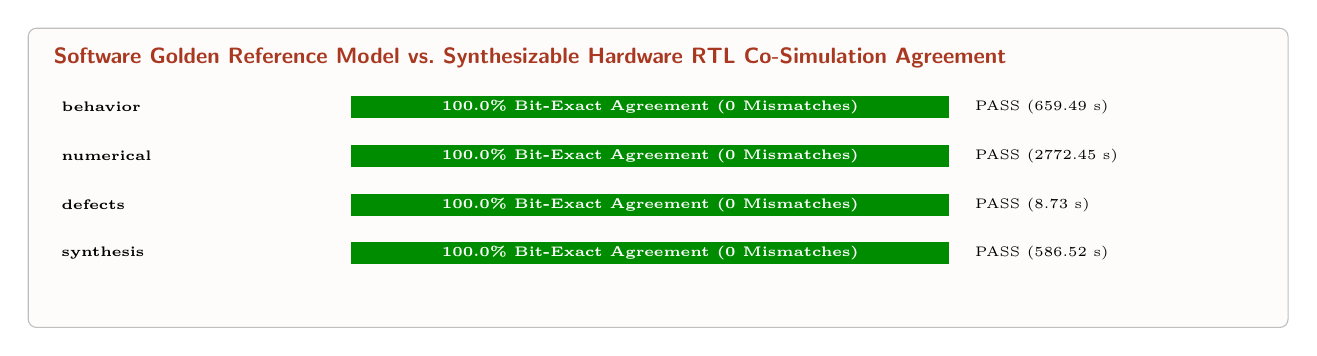
\begin{tikzpicture}[font=\scriptsize\sffamily]

\draw[draw=black!25,fill=vulcan!2,rounded corners=3pt] (-0.5,-1.85) rectangle (15.5,1.95);

\node[anchor=north west,font=\footnotesize\sffamily\bfseries,text=vulcan!90!black] at (-0.3,1.82) {Software Golden Reference Model vs.\ Synthesizable Hardware RTL Co-Simulation Agreement};

\node[anchor=west,font=\tiny\bfseries] at (-0.2,0.95) {behavior};

\fill[green!55!black] (3.6,0.81) rectangle (11.2,1.09);

\node[text=white,font=\tiny\bfseries] at (7.4,0.95) {100.0\% Bit-Exact Agreement (0 Mismatches)};

\node[anchor=west,font=\tiny] at (11.4,0.95) {PASS (659.49 s)};

\node[anchor=west,font=\tiny\bfseries] at (-0.2,0.33) {numerical};

\fill[green!55!black] (3.6,0.19) rectangle (11.2,0.47);

\node[text=white,font=\tiny\bfseries] at (7.4,0.33) {100.0\% Bit-Exact Agreement (0 Mismatches)};

\node[anchor=west,font=\tiny] at (11.4,0.33) {PASS (2772.45 s)};

\node[anchor=west,font=\tiny\bfseries] at (-0.2,-0.29) {defects};

\fill[green!55!black] (3.6,-0.43) rectangle (11.2,-0.15);

\node[text=white,font=\tiny\bfseries] at (7.4,-0.29) {100.0\% Bit-Exact Agreement (0 Mismatches)};

\node[anchor=west,font=\tiny] at (11.4,-0.29) {PASS (8.73 s)};

\node[anchor=west,font=\tiny\bfseries] at (-0.2,-0.91) {synthesis};

\fill[green!55!black] (3.6,-1.05) rectangle (11.2,-0.77);

\node[text=white,font=\tiny\bfseries] at (7.4,-0.91) {100.0\% Bit-Exact Agreement (0 Mismatches)};

\node[anchor=west,font=\tiny] at (11.4,-0.91) {PASS (586.52 s)};

\end{tikzpicture}\par

{\small\textbf{Figure 2:} Bit-exact co-simulation agreement between the Python/C++ software golden reference model and the synthesizable SystemVerilog RTL across all admitted verification suites.}\end{center}

\subsection{Unified Hardware Signoff Gates (L1 Lint, L2 Quartus STA, L3 Physical FPGA)}

{\small\renewcommand{\arraystretch}{1.18}\begin{longtable}{@{}L{0.34\textwidth}L{0.12\textwidth}L{0.46\textwidth}@{}}\toprule

\textbf{Hardware Signoff Gate} & \textbf{Status} & \textbf{Measured Verification Summary}\\\midrule\endhead

L1 Static RTL Timing \& Synthesis Lint & PASSED & Combinational div/\allowbreak{}mod hazards: 0; mixed sequential assignments (\allowbreak{}10268)\allowbreak{}: 0\\[3pt]

\bottomrule\end{longtable}}

\section{Integration and use}

Use \texttt{rtl/\allowbreak{}*\allowbreak{}.sv} with top \texttt{billet\_\allowbreak{}f3\_\allowbreak{}top}. Consult \texttt{design/\allowbreak{}SPEC.md},\allowbreak{} \texttt{design/\allowbreak{}ARCHITECTURE.md} and \texttt{tests/\allowbreak{}METHOD.md}. Do not co-compile duplicate parent module definitions from both RTL trees.


Assert reset before traffic. Fully program and commit each required channel's inactive banks,\allowbreak{} then handshake a legal chain descriptor. Reset coefficients are zero. Legacy integration ties \texttt{sos\_\allowbreak{}cfg\_\allowbreak{}valid},\allowbreak{} \texttt{sos\_\allowbreak{}commit\_\allowbreak{}valid} and \texttt{chain\_\allowbreak{}valid} low and all associated request fields to zero.


Withdraw incomplete commit requests before supplying missing writes: any update-valid blocks staging writes. Hold requests through backpressure,\allowbreak{} and eventually withdraw invalid descriptors or incomplete updates to avoid deliberate input blockage.


Prerequisites are Python 3 with standard library,\allowbreak{} \texttt{iverilog},\allowbreak{} \texttt{vvp} and \texttt{yosys} on PATH. Recorded versions were Python 3.12.3,\allowbreak{} Icarus 12.0 and Yosys 0.33. No dependency installation is performed.


From the project root,\allowbreak{} run the full suite with \texttt{python3 tests/\allowbreak{}verify.py}. Individual commands are \texttt{python3 tests/\allowbreak{}verify.py --check behavior},\allowbreak{} \texttt{python3 tests/\allowbreak{}verify.py --check numerical},\allowbreak{} \texttt{python3 tests/\allowbreak{}verify.py --check defects},\allowbreak{} \texttt{python3 tests/\allowbreak{}verify.py --check synthesis} and \texttt{python3 tests/\allowbreak{}verify.py --check portable}. The last command is the executed bounded clean-directory subset,\allowbreak{} not the full matrix.


Each \texttt{evidence/\allowbreak{}<check>/\allowbreak{}results.json} indexes retained runs with source hashes,\allowbreak{} configurations,\allowbreak{} seeds,\allowbreak{} measured counts,\allowbreak{} exact child commands and raw-result receipts. Generated evidence is not a build input; preserve failed runs when reproducing.


\section{Limitations and acceptance boundary}

Stability and numerical-error conclusions apply only to the declared quantized fixtures and tested stimulus conditions. Arbitrary user coefficients can saturate,\allowbreak{} diverge or exhibit limit cycles; zero external decay residual does not imply zero internal recursive state.


FIR coefficient 32767 represents 32767/\allowbreak{}32768,\allowbreak{} not exact unity. Quantization and saturation can make the two mixed orders observably different.


The chain is global,\allowbreak{} with one FIR instance and an ascending SOS prefix. Per-channel descriptors,\allowbreak{} repeated FIR blocks,\allowbreak{} arbitrary routing lists,\allowbreak{} multiple outstanding samples,\allowbreak{} clock-domain crossing and a software register bus are unsupported.


Invalid descriptors and incomplete updates intentionally exert backpressure rather than returning an error response. Integrators are responsible for control-producer liveness and reset-release discipline.


No physical area,\allowbreak{} timing closure,\allowbreak{} FPGA measurements,\allowbreak{} silicon-security result or formal proof is claimed. Generic synthesis statistics and cycle schedules do not establish an achievable clock frequency.


\appendix\section{Source inventory}

Production inventory: 9 Verilog/\allowbreak{}SystemVerilog files; 887 nonblank,\allowbreak{} non-comment lines. Source size is not a correctness or quality metric.

{\small\renewcommand{\arraystretch}{1.18}\begin{longtable}{@{}L{0.61\textwidth}L{0.15\textwidth}L{0.15\textwidth}@{}}\toprule

\textbf{Production file} & \textbf{Physical lines} & \textbf{Code lines}\\\midrule\endhead

rtl/\allowbreak{}billet\_\allowbreak{}f2\_\allowbreak{}coeff\_\allowbreak{}bank.sv & 66 & 62\\[3pt]

rtl/\allowbreak{}billet\_\allowbreak{}f2\_\allowbreak{}history.sv & 42 & 38\\[3pt]

rtl/\allowbreak{}billet\_\allowbreak{}f2\_\allowbreak{}mac.sv & 79 & 73\\[3pt]

rtl/\allowbreak{}billet\_\allowbreak{}f2\_\allowbreak{}round\_\allowbreak{}sat.sv & 32 & 28\\[3pt]

rtl/\allowbreak{}billet\_\allowbreak{}f2\_\allowbreak{}top.sv & 149 & 141\\[3pt]

rtl/\allowbreak{}billet\_\allowbreak{}f3\_\allowbreak{}round\_\allowbreak{}sat.sv & 29 & 26\\[3pt]

rtl/\allowbreak{}billet\_\allowbreak{}f3\_\allowbreak{}sos\_\allowbreak{}coeff\_\allowbreak{}bank.sv & 79 & 75\\[3pt]

rtl/\allowbreak{}billet\_\allowbreak{}f3\_\allowbreak{}sos\_\allowbreak{}engine.sv & 208 & 201\\[3pt]

rtl/\allowbreak{}billet\_\allowbreak{}f3\_\allowbreak{}top.sv & 252 & 243\\[3pt]

\bottomrule\end{longtable}}

\section{Verification record index}

{\small\renewcommand{\arraystretch}{1.18}\begin{longtable}{@{}L{0.57\textwidth}L{0.16\textwidth}L{0.17\textwidth}@{}}\toprule

\textbf{Recorded check} & \textbf{Outcome} & \textbf{Execution time (\allowbreak{}s)\allowbreak{}}\\\midrule\endhead

behavior & passed & 659.488\\[3pt]

numerical & passed & 2772.445\\[3pt]

defects & passed & 8.733\\[3pt]

synthesis & passed & 586.516\\[3pt]

portable & passed & 111.216\\[3pt]

\bottomrule\end{longtable}}

Execution times include tool and provider waiting; they are not hardware latency or model utilization.

{\small\renewcommand{\arraystretch}{1.18}\begin{longtable}{@{}L{0.12\textwidth}L{0.82\textwidth}@{}}\toprule

\textbf{Reference} & \textbf{Original project-relative record}\\\midrule\endhead

E012 & tests/\allowbreak{}METHOD.md\\[3pt]

E016 & tests/\allowbreak{}bridge.sv\\[3pt]

E017 & tests/\allowbreak{}model.py\\[3pt]

E018 & tests/\allowbreak{}round\_\allowbreak{}bridge.sv\\[3pt]

E019 & tests/\allowbreak{}verify.py\\[3pt]

E020 & tests/\allowbreak{}workloads.py\\[3pt]

E029 & .vulcan/\allowbreak{}engineering/\allowbreak{}run-0001/\allowbreak{}attempt-0008/\allowbreak{}stdout.log\\[3pt]

E030 & .vulcan/\allowbreak{}engineering/\allowbreak{}run-0001/\allowbreak{}attempt-0009/\allowbreak{}response.json\\[3pt]

E031 & .vulcan/\allowbreak{}engineering/\allowbreak{}run-0001/\allowbreak{}attempt-0010/\allowbreak{}stdout.log\\[3pt]

E032 & .vulcan/\allowbreak{}engineering/\allowbreak{}run-0001/\allowbreak{}attempt-0011/\allowbreak{}stdout.log\\[3pt]

E033 & .vulcan/\allowbreak{}engineering/\allowbreak{}run-0001/\allowbreak{}attempt-0012/\allowbreak{}stdout.log\\[3pt]

E034 & .vulcan/\allowbreak{}engineering/\allowbreak{}run-0001/\allowbreak{}attempt-0013/\allowbreak{}stdout.log\\[3pt]

E035 & .vulcan/\allowbreak{}engineering/\allowbreak{}run-0001/\allowbreak{}attempt-0014/\allowbreak{}stdout.log\\[3pt]

\bottomrule\end{longtable}}

\section{Document provenance}

Engineering was independently accepted for the recorded source and evidence identity. This is not exhaustive proof, hardware deployment or physical signoff. The companion REPORT.md records the exact report approval and source manifest, and links the English/Chinese journeys containing original failures and interventions. A report number identifies a generation attempt, not a new hardware revision.

Developer attribution is explicitly supplied project metadata, not inferred affiliation or institutional endorsement.

\end{document}
